\section{Introduction}
This chapter presents the architecture and design of RV32ICore, a pipelined 32-bit RISC-V processor implementing the RV32I Base Integer ISA. The chapter begins with a top-level overview of the processor's major units, followed by a detailed description of each pipeline stage, the pipeline registers connecting them, and the hazard unit responsible for maintaining correct execution in the presence of data and control hazards.

\section{Top-Level Architecture}
At the highest level of abstraction, RV32ICore is composed of two primary units: the Datapath and the Control Unit, along with a dedicated Hazard Unit that operates across pipeline stages.

\textbf{The Datapath} is responsible for processing and routing data throughout the processor. Its inputs include control signals generated by the Control Unit, instructions fetched from instruction memory, and data read from data memory. Its outputs include the Program Counter (PC) supplied to instruction memory, data written to data memory, and status information such as instruction fields and condition flags fed back to the Control Unit.

\textbf{The Control Unit} is responsible for managing the correct execution of instructions by interpreting instruction fields and generating the appropriate control signals for each pipeline stage. Its inputs are the opcode (bits [6:0]), Funct3 (bits [14:12]), and Funct7 bit 30, along with the processor clock and reset. Its outputs are the set of control signals that govern the behavior of multiplexers, the register file, the ALU, and the data memory throughout the datapath.

\textbf{The Hazard Unit} monitors the pipeline state and intervenes when hazard conditions are detected. It generates stall and flush signals to preserve correct program execution in the presence of data dependencies and control flow changes. Its operation is described in detail in Section 3.9.
\begin{figure}[h!]
    \centering
    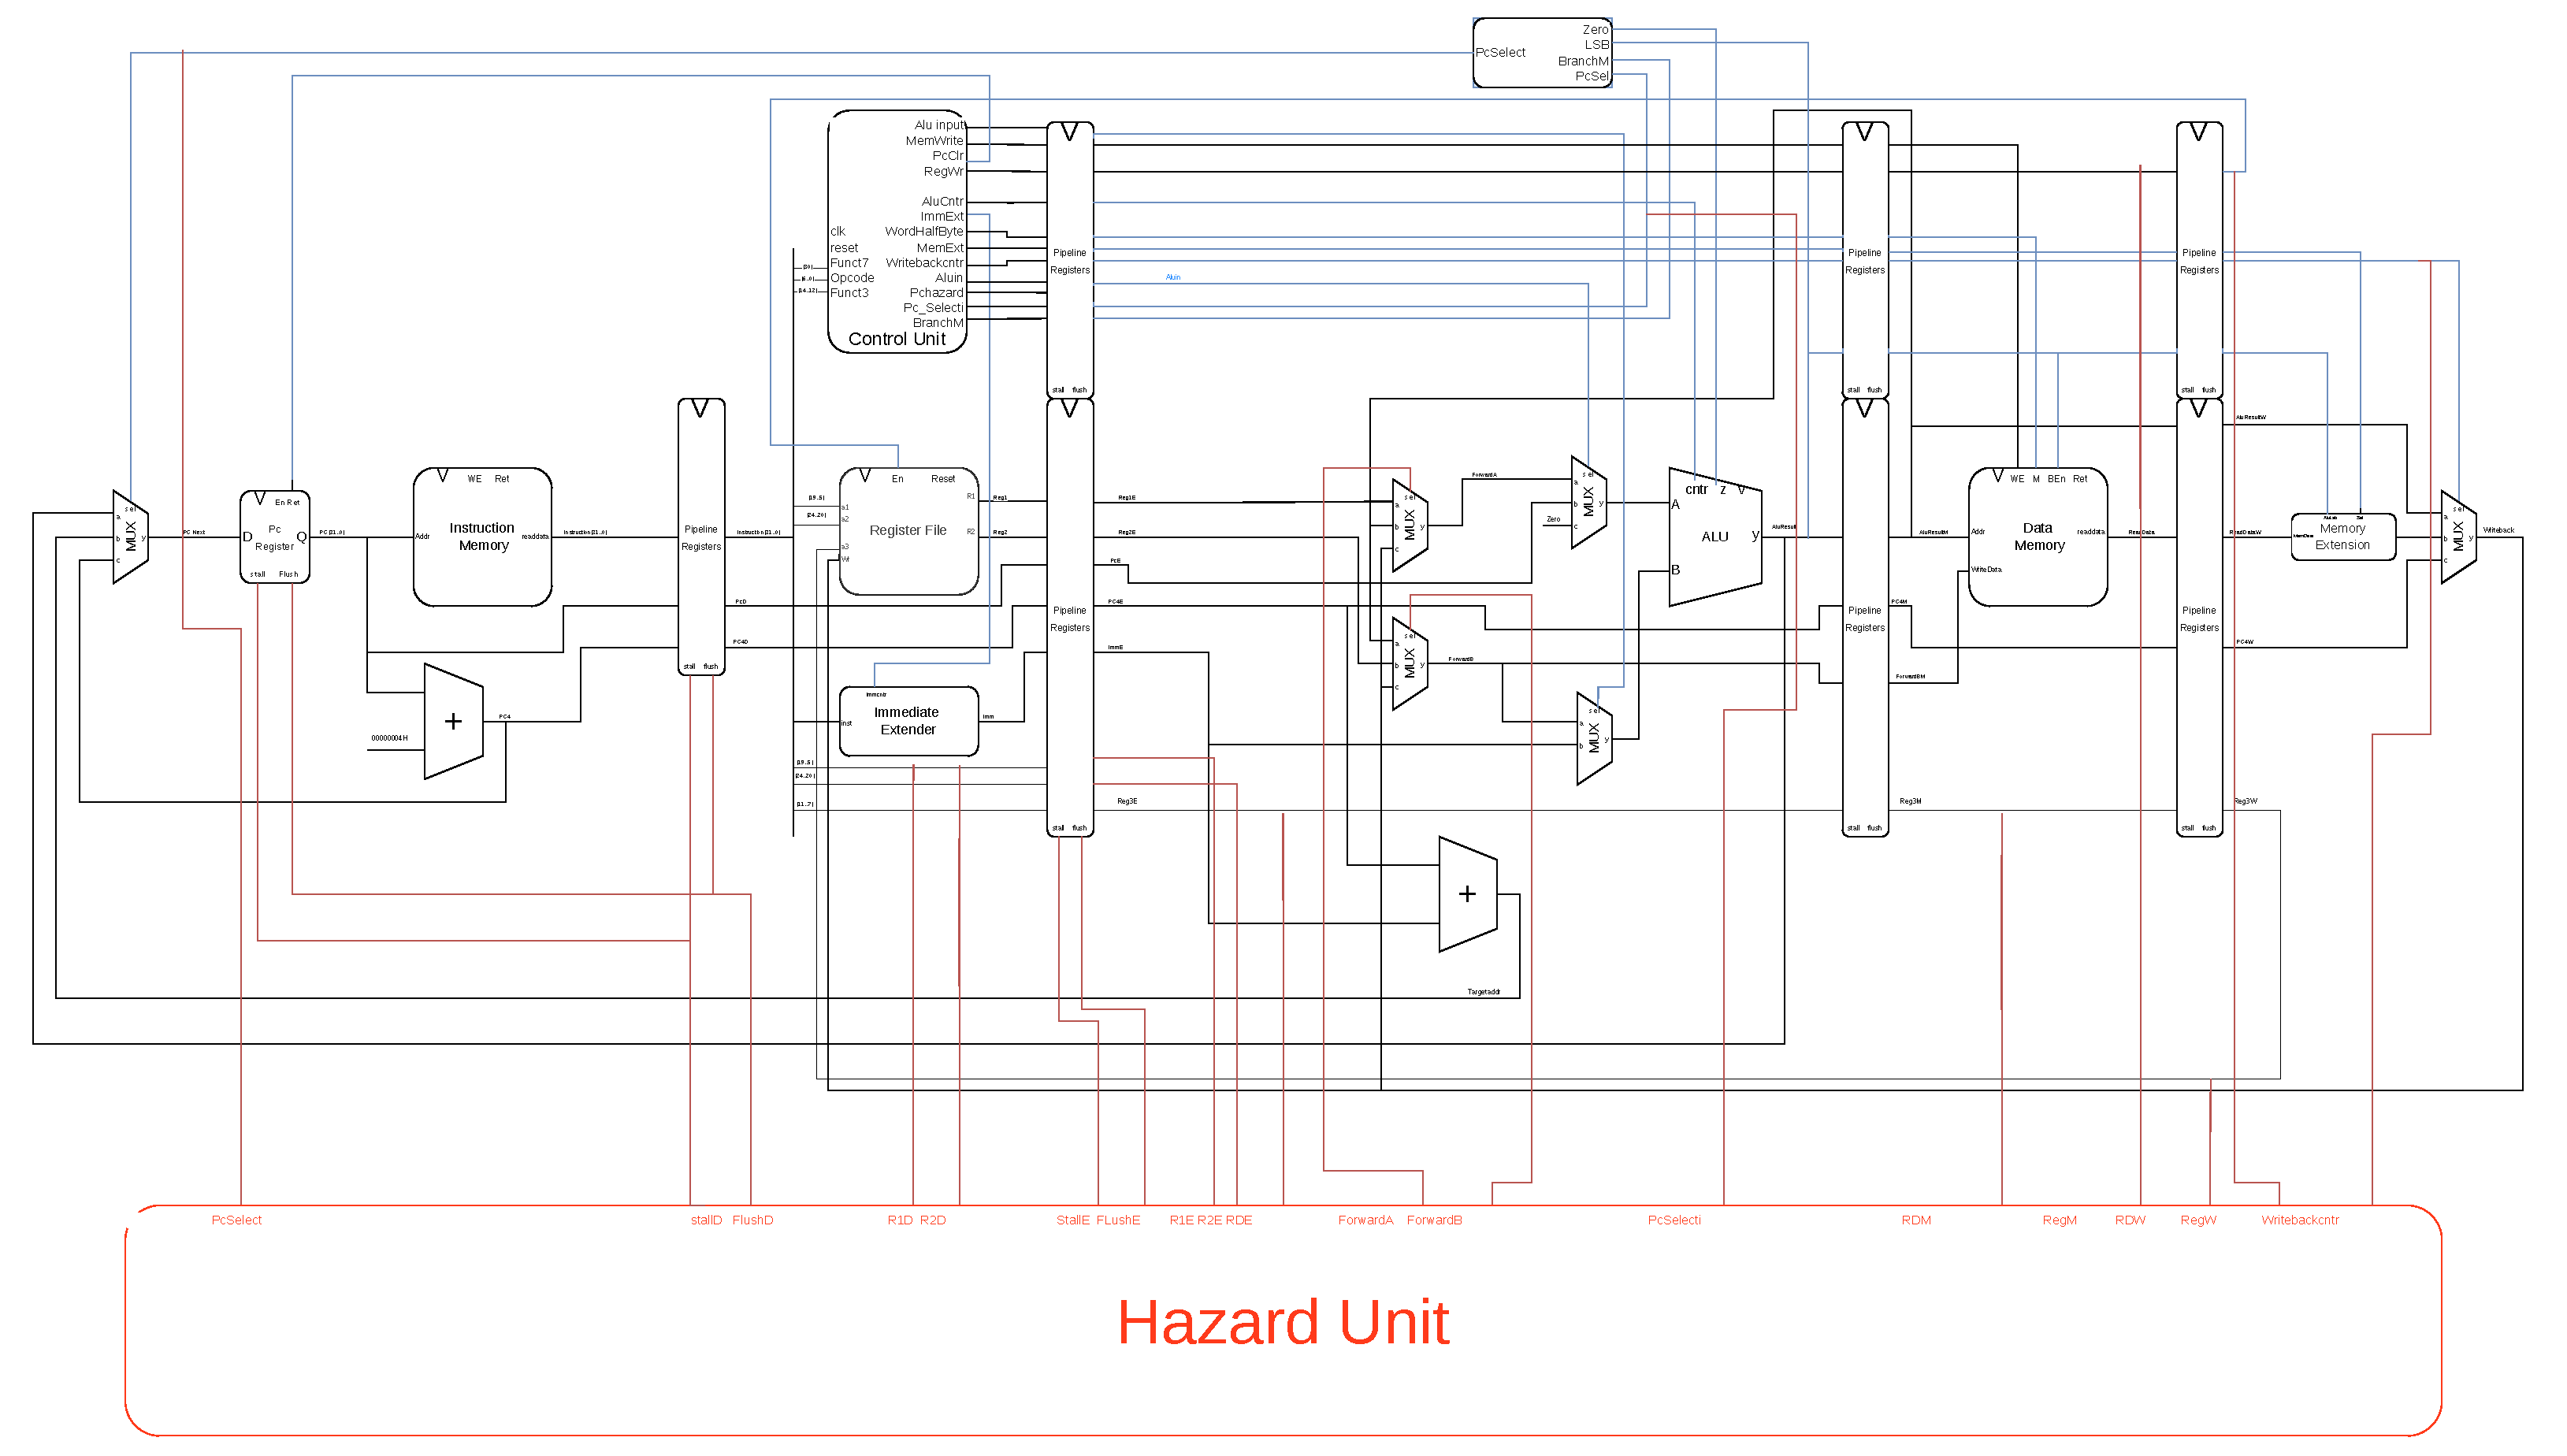
\includegraphics[scale=0.3]{Figures/Chapter 3/Top Level.pdf}
    \caption{RV32ICore Top-Level Architecture}
    \label{fig: RV32ICore Top-Level Architecture}
\end{figure}
\section{Pipeline Overview}
RV32ICore implements a classical five-stage pipeline. Pipelining allows multiple instructions to be in different stages of execution simultaneously, improving throughput by overlapping work across stages. The five stages are:

\begin{itemize}
    \item \textbf{IF} — Instruction Fetch
    \item \textbf{ID} — Instruction Decode
    \item \textbf{EX} — Execute
    \item \textbf{MEM} — Memory Access
    \item \textbf{WB} — Write-Back
\end{itemize}

Each stage is separated from the next by a pipeline register that captures the outputs of the current stage and holds them stable for the following stage on the next clock edge. All pipeline registers share the same clock as the rest of the processor and are controlled by two signals: a synchronous reset that clears the register to zero, and a NOP insertion signal that loads a harmless no-operation instruction into the register without clearing its other fields, used during flush operations.
\section{Instruction Fetch (IF) Stage}
The Instruction Fetch stage is responsible for retrieving the current instruction from instruction memory and advancing the Program Counter

The PC is stored in a dedicated register that updates on every rising clock edge under normal operation. Its value is used directly as the address supplied to the instruction memory, which responds combinationally with the 32-bit instruction word stored at that address.

A dedicated adder computes PC+4, representing the address of the next sequential instruction. This value is carried forward through the pipeline and is used in the Write-Back stage as the return address for jump instructions.

On a taken branch, the PC is updated to the branch target address computed in the Execute stage in the same cycle that the flush signal is issued. Under normal sequential execution, the PC is updated to PC+4.

The instruction memory is separate from the data memory, consistent with the Harvard architecture adopted by RV32ICore. This ensures that instruction fetch never contends with data memory access, eliminating structural hazards between the IF and MEM stages.
\begin{figure}[h!]
    \centering
    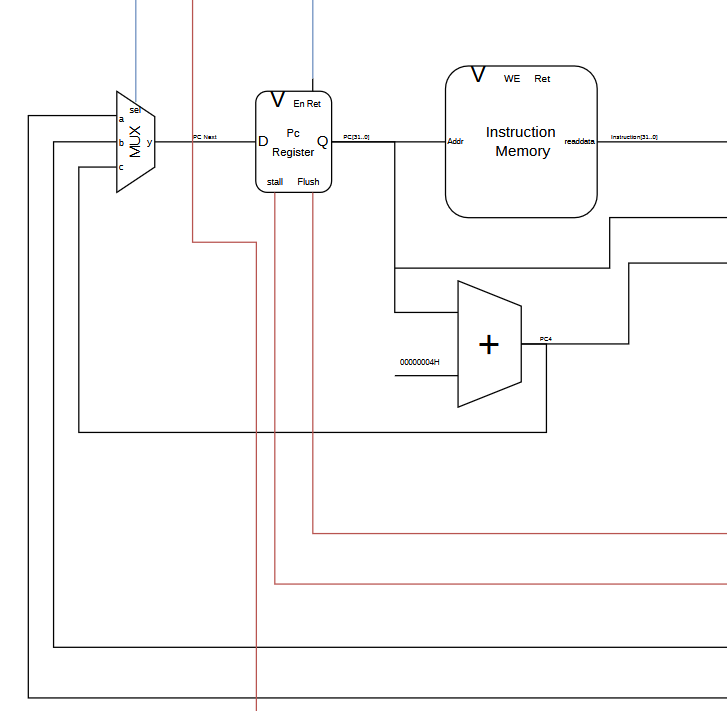
\includegraphics[scale=0.3]{Figures/Chapter 3/IF Stage.png}
    \caption{RV32ICore IF Stage}
    \label{fig: RV32ICore IF Stage}
\end{figure}
\section{Instruction Decode (ID) Stage}
The Instruction Decode stage deconstructs the fetched instruction and prepares the operands and control signals required for execution.

The 32-bit instruction word is partitioned into its constituent fields according to the RV32I specification. The source register addresses rs1 and rs2 are located at bits [19:15] and [24:20] respectively, and the destination register address rd is located at bits [11:7]. These addresses are wired directly to the read ports of the register file, which responds combinationally with the contents of the addressed registers. Register x0 is hardwired to zero; any read of x0 returns zero and any write to x0 is silently discarded.

An Immediate Extension unit receives the full 32-bit instruction word and produces a 32-bit sign-extended immediate value. The extension logic selects the appropriate immediate format — I, S, B, U, or J — based on the opcode, and assembles the immediate from the relevant instruction bits according to the RV32I encoding specification.

The opcode (bits [6:0]), Funct3 (bits [14:12]), and Funct7 bit 30 are forwarded to the Control Unit, which decodes them and generates the full set of control signals for the instruction. These control signals are stored in the ID/EX pipeline register alongside the register data and immediate value and propagate through the pipeline with the instruction.
\begin{figure}[h!]
    \centering
    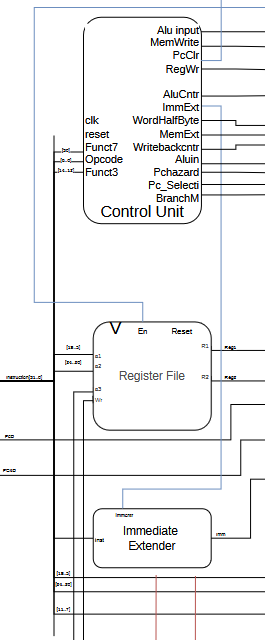
\includegraphics[scale=0.3]{Figures/Chapter 3/ID Stage.png}
    \caption{RV32ICore ID Stage}
    \label{fig: RV32ICore ID Stage}
\end{figure}
\section{Execute (EX) Stage}
The Execute stage performs the arithmetic, logical, or address computation required by the current instruction. It is the most complex stage of the datapath, containing the ALU, two input multiplexers, a branch adder, and the forwarding multiplexer logic.
\subsection{ALU Input Selection}
Two multiplexers select the operands presented to the ALU inputs.

\textbf{MuxX3} selects ALU input A from three possible sources: the value of register rs1, the current PC (used by AUIPC), or zero (used by LUI, which adds the upper immediate to zero so that the ALU result path is reused without requiring dedicated hardware). The selection is governed by a control signal generated by the Control Unit.

\textbf{MuxX2} selects ALU input B from two possible sources: the value of register rs2 (for register-to-register instructions) or the sign-extended immediate (for immediate-type instructions). The selection is governed by a corresponding control signal.

\subsection{ALU Operation}
The ALU receives the two selected operands and performs the operation specified by the ALU control signal, which is derived from the opcode, Funct3, and Funct7 fields decoded in the Control Unit. Supported operations include addition, subtraction, bitwise AND, OR, and XOR, logical and arithmetic shift, and signed and unsigned comparison. The ALU produces a 32-bit result and a zero flag used for branch condition evaluation.
\subsection{Branch Address Computation}
A dedicated adder computes the branch target address by summing the PC value carried from the IF stage with the sign-extended immediate. This target address is passed to the PC register when a branch is taken.
\subsection{Branch Resolution}
Branch conditions are evaluated in the Execute stage. When a branch is taken, the Hazard Unit issues a flush signal that inserts NOP instructions into the IF/ID and ID/EX pipeline registers in the same cycle that the PC is updated to the branch target. This discards the two incorrectly fetched instructions that entered the pipeline after the branch. No branch prediction is employed; the pipeline always flushes on a taken branch.
\begin{figure}[h!]
    \centering
    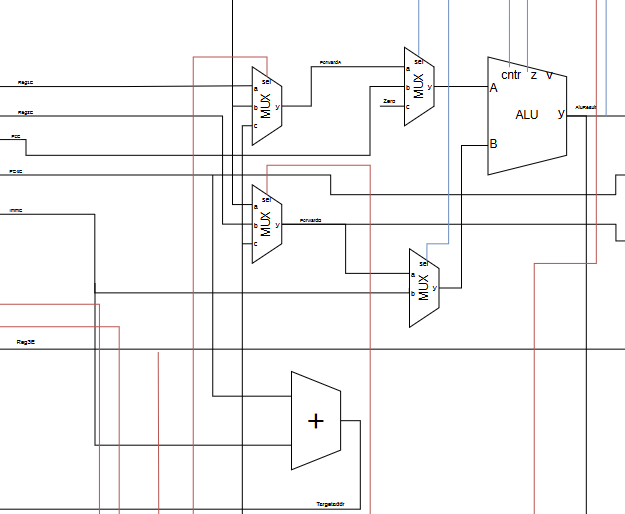
\includegraphics[scale=0.3]{Figures/Chapter 3/EX Stage.png}
    \caption{RV32ICore EX Stage}
    \label{fig:RV32ICore RV32ICore EX Stage}
\end{figure}
\section{Memory Access (MEM) Stage}
The Memory Access stage handles Load and Store instructions by interfacing with the data memory.

For Store instructions, the address computed by the ALU in the Execute stage is used as the write address, and the value of register rs2 — carried through the pipeline — is written to data memory. For Load instructions, the same computed address is used as the read address, and the data memory responds with the value stored at that location.

The data memory supports three access widths controlled by a signal derived from the Funct3 field: byte (8-bit), halfword (16-bit), and word (32-bit). For instructions that do not access memory, this stage passes the ALU result and control signals through to the Write-Back stage without interacting with the data memory.
\begin{figure}[h!]
    \centering
    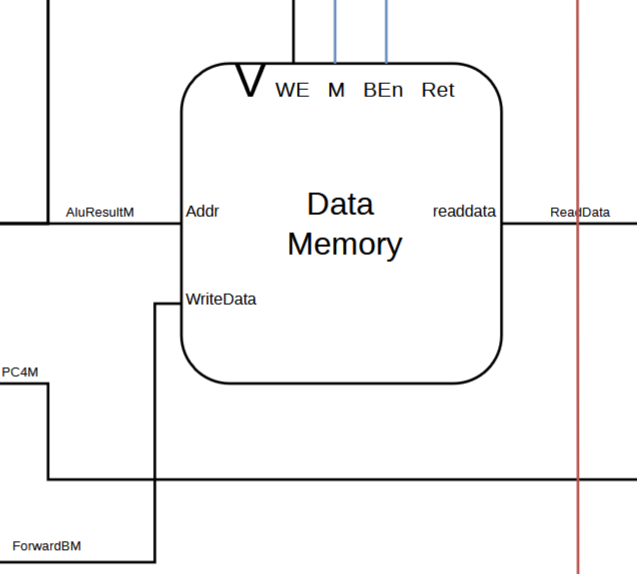
\includegraphics[scale=0.3]{Figures/Chapter 3/MEM Stage.png}
    \caption{RV32ICore MEM Stage}
    \label{fig:RV32ICore MEM Stage}
\end{figure}
\section{Write-Back (WB) Stage}
The Write-Back stage selects the value to be written to the destination register and commits it to the register file.

A Memory Extension unit first processes the raw data returned by the data memory. It performs sign extension or zero extension of byte and halfword values according to the access type specified by the Funct3 field, ensuring that the value written to the 32-bit register file conforms to the RV32I specification for load instructions.

A multiplexer then selects among three possible write-back sources: the ALU result (for arithmetic, logical, and address computation instructions), the extended memory data (for load instructions), and PC+4 (for JAL and JALR, which write the return address to the destination register). The selected value is written to the register file at the address specified by rd on the rising clock edge, completing the instruction's execution.
\begin{figure}[h!]
    \centering
    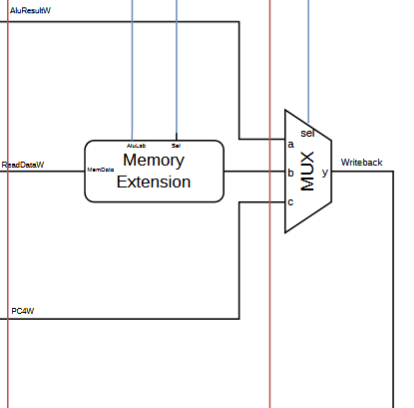
\includegraphics[scale=0.3]{Figures/Chapter 3/WR Stage.png}
    \caption{RV32ICore WR Stage}
    \label{fig:RV32ICore WR Stage}
\end{figure}
\section{Hazard Unit}
The Hazard Unit monitors the pipeline registers and intervenes when conditions arise that would cause incorrect execution. It handles three categories of hazards: data hazards, load-use hazards, and control hazards.

\subsection{Data Hazards and Forwarding}
Data hazards occur when an instruction depends on the result of a preceding instruction that has not yet been written back to the register file. RV32ICore resolves most data hazards through forwarding, which routes computed results directly from later pipeline stages back to the ALU inputs in the Execute stage, bypassing the register file.

The Hazard Unit compares the destination register of instructions in the EX/MEM and MEM/WB pipeline registers against the source registers of the instruction currently in the Execute stage. When a match is detected, forwarded values are selected at both MuxX2 and MuxX3 in place of the register file outputs. When forwarding from the MEM/WB stage following a load instruction, the forwarded value is taken from the output of the Memory Extension unit, ensuring that the correctly sign-extended loaded value is used.
\subsection{Load-Use Hazards}
A load-use hazard occurs when a load instruction is immediately followed by an instruction that uses the loaded value. Since the loaded data is not available until the end of the Memory Access stage, forwarding alone cannot resolve this hazard. The Hazard Unit detects this condition by checking whether the instruction in the Execute stage is a load and whether its destination register matches a source register of the instruction in the Decode stage. When detected, the Hazard Unit stalls the pipeline for one cycle by freezing the IF/ID and ID/EX pipeline registers and inserting a NOP into the Execute stage, allowing the loaded value to reach the MEM/WB stage where it can be forwarded.
\subsection{Control Hazards}
Control hazards arise from branch and jump instructions, whose target addresses are not known until the Execute stage. Since two instructions are fetched after every branch before its outcome is resolved, those instructions must be discarded if the branch is taken. The Hazard Unit handles this by issuing a flush signal that inserts NOP instructions into the IF/ID and ID/EX pipeline registers in the same cycle that the PC is updated to the branch target address.
\begin{figure}[h!]
    \centering
    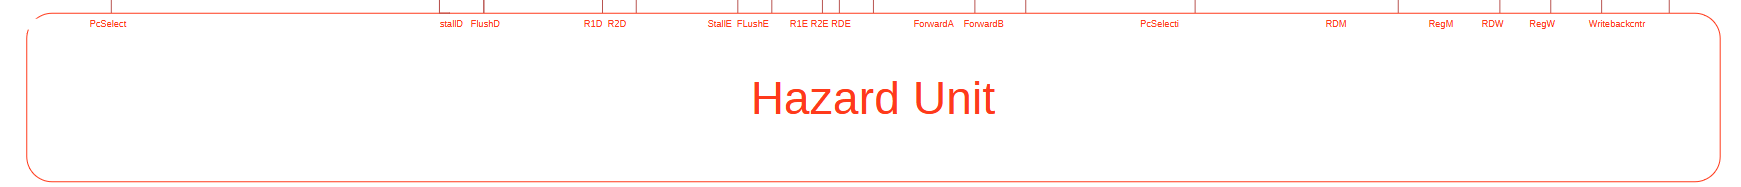
\includegraphics[scale=0.3]{Figures/Chapter 3/Hazard Unit.png}
    \caption{RV32ICore Hazard Unit}
    \label{fig:RV32ICore Hazard Unit}
\end{figure}
\section{Conclusion}
This chapter has presented the complete architecture of RV32ICore, covering its top-level decomposition into Datapath, Control Unit, and Hazard Unit, and providing a detailed description of each pipeline stage and the registers connecting them. The five-stage Harvard pipeline provides a structured and efficient framework for RV32I instruction execution. The forwarding and stalling mechanisms implemented in the Hazard Unit ensure correct execution in the presence of data dependencies, while pipeline flushing resolves control hazards introduced by branch and jump instructions. The architectural decisions described in this chapter form the direct basis for the VHDL implementation presented in the following chapter.
